\documentclass{sigchi}

% Use this section to set the ACM copyright statement (e.g. for
% preprints).  Consult the conference website for the camera-ready
% copyright statement.

% Copyright
\CopyrightYear{2020}
%\setcopyright{acmcopyright}
\setcopyright{acmlicensed}
%\setcopyright{rightsretained}
%\setcopyright{usgov}
%\setcopyright{usgovmixed}
%\setcopyright{cagov}
%\setcopyright{cagovmixed}
% DOI
\doi{https://doi.org/10.1145/3313831.XXXXXXX}
% ISBN
\isbn{978-1-4503-6708-0/20/04}
%Conference
\conferenceinfo{CHI'20,}{April  25--30, 2020, Honolulu, HI, USA}
%Price
\acmPrice{\$15.00}

% Use this command to override the default ACM copyright statement
% (e.g. for preprints).  Consult the conference website for the
% camera-ready copyright statement.

%% HOW TO OVERRIDE THE DEFAULT COPYRIGHT STRIP --
%% Please note you need to make sure the copy for your specific
%% license is used here!
% \toappear{
% Permission to make digital or hard copies of all or part of this work
% for personal or classroom use is granted without fee provided that
% copies are not made or distributed for profit or commercial advantage
% and that copies bear this notice and the full citation on the first
% page. Copyrights for components of this work owned by others than ACM
% must be honored. Abstracting with credit is permitted. To copy
% otherwise, or republish, to post on servers or to redistribute to
% lists, requires prior specific permission and/or a fee. Request
% permissions from \href{mailto:Permissions@acm.org}{Permissions@acm.org}. \\
% \emph{CHI '16},  May 07--12, 2016, San Jose, CA, USA \\
% ACM xxx-x-xxxx-xxxx-x/xx/xx\ldots \$15.00 \\
% DOI: \url{http://dx.doi.org/xx.xxxx/xxxxxxx.xxxxxxx}
% }

% Arabic page numbers for submission.  Remove this line to eliminate
% page numbers for the camera ready copy
% \pagenumbering{arabic}

% Load basic packages
\usepackage{balance}       % to better equalize the last page
\usepackage{graphics}      % for EPS, load graphicx instead 
\usepackage[T1]{fontenc}   % for umlauts and other diaeresis
\usepackage{txfonts}
\usepackage{mathptmx}
\usepackage[pdflang={en-US},pdftex]{hyperref}
\usepackage{color}
\usepackage{booktabs}
\usepackage{textcomp}

% Some optional stuff you might like/need.
\usepackage{microtype}        % Improved Tracking and Kerning
% \usepackage[all]{hypcap}    % Fixes bug in hyperref caption linking
\usepackage{ccicons}          % Cite your images correctly!
% \usepackage[utf8]{inputenc} % for a UTF8 editor only

% If you want to use todo notes, marginpars etc. during creation of
% your draft document, you have to enable the "chi_draft" option for
% the document class. To do this, change the very first line to:
% "\documentclass[chi_draft]{sigchi}". You can then place todo notes
% by using the "\todo{...}"  command. Make sure to disable the draft
% option again before submitting your final document.
\usepackage{todonotes}

% Paper metadata (use plain text, for PDF inclusion and later
% re-using, if desired).  Use \emtpyauthor when submitting for review
% so you remain anonymous.
\def\plaintitle{Explore, Edit, Guess: Understanding Novice Programmers' Use of Codeblocks for Regression Experiments}
\def\plainauthor{First Author, Second Author, Third Author,
  Fourth Author, Fifth Author, Sixth Author}
\def\emptyauthor{}
\def\plainkeywords{Machine Learning; Codeblocks Programming; Novice Programmer Practices; Interactive Machine Learning}
\def\plaingeneralterms{Programming}

% llt: Define a global style for URLs, rather that the default one
\makeatletter
\def\url@leostyle{%
  \@ifundefined{selectfont}{
    \def\UrlFont{\sf}
  }{
    \def\UrlFont{\small\bf\ttfamily}
  }}
\makeatother
\urlstyle{leo}

% To make various LaTeX processors do the right thing with page size.
\def\pprw{8.5in}
\def\pprh{11in}
\special{papersize=\pprw,\pprh}
\setlength{\paperwidth}{\pprw}
\setlength{\paperheight}{\pprh}
\setlength{\pdfpagewidth}{\pprw}
\setlength{\pdfpageheight}{\pprh}

% Make sure hyperref comes last of your loaded packages, to give it a
% fighting chance of not being over-written, since its job is to
% redefine many LaTeX commands.
\definecolor{linkColor}{RGB}{6,125,233}
\hypersetup{%
  pdftitle={\plaintitle},
% Use \plainauthor for final version.
%  pdfauthor={\plainauthor},
  pdfauthor={\emptyauthor},
  pdfkeywords={\plainkeywords},
  pdfdisplaydoctitle=true, % For Accessibility
  bookmarksnumbered,
  pdfstartview={FitH},
  colorlinks,
  citecolor=black,
  filecolor=black,
  linkcolor=black,
  urlcolor=linkColor,
  breaklinks=true,
  hypertexnames=false
}

% create a shortcut to typeset table headings
% \newcommand\tabhead[1]{\small\textbf{#1}}

% End of preamble. Here it comes the document.
\begin{document}

\title{\plaintitle}

\numberofauthors{3}
\author{%
  \alignauthor{Leave Authors Anonymous\\
    \affaddr{for Submission}\\
    \affaddr{City, Country}\\
    \email{e-mail address}}\\
  \alignauthor{Leave Authors Anonymous\\
    \affaddr{for Submission}\\
    \affaddr{City, Country}\\
    \email{e-mail address}}\\
  \alignauthor{Leave Authors Anonymous\\
    \affaddr{for Submission}\\
    \affaddr{City, Country}\\
    \email{e-mail address}}\\
}

\maketitle

\begin{abstract}
%  
Machine Learning (ML) suites are readily-available for practical use. There are available packaged software and console libraries that can be modified. However, novice programmers avoid these ML suites due to the abstractions with pre-existing tools. Users with limited programming background that know how these models work, struggle with converting them to code for practical use. We iterated on developing a codeblocks tool for linear regression tasks where we did multiple usability tests involving 33 participants. We observed how they went through their ML tasks, and inquired into their pains and struggles in writing code. Experienced programmers typically follow the Edit-Explore-Guess activity flow. In contrast, we found novices that struggle with code tend to follow Explore-Edit-Guess flow wherein they explore their environment before they gain more confidence with building code. We conclude by deriving design guidelines to provide affordances that cater to their needs.
\end{abstract}
% ACM Classfication

\begin{CCSXML}
<ccs2012>
<concept>
<concept_id>10003120.10003121</concept_id>
<concept_desc>Human-centered computing~Human computer interaction (HCI)</concept_desc>
<concept_significance>500</concept_significance>
</concept>
<concept>
<concept_id>10003120.10003121.10003125.10011752</concept_id>
<concept_desc>Human-centered computing~Haptic devices</concept_desc>
<concept_significance>300</concept_significance>
</concept>
<concept>
<concept_id>10003120.10003121.10003122.10003334</concept_id>
<concept_desc>Human-centered computing~User studies</concept_desc>
<concept_significance>100</concept_significance>
</concept>
</ccs2012>
\end{CCSXML}

\ccsdesc[500]{Human-centered computing~Human computer interaction (HCI)}
\ccsdesc[300]{Human-centered computing~Haptic devices}
\ccsdesc[100]{Human-centered computing~User studies}

% Author Keywords
\keywords{\plainkeywords}

% Print the classficiation codes
\printccsdesc
Please use the 2012 Classifiers and see this link to embed them in the text: \url{https://dl.acm.org/ccs/ccs_flat.cfm}

\section{Introduction}
Several Machine Learning (ML) applications and programs have been made readily-available for various types of users and use-cases. These applications are made accessible towards having a wider-spread of use of ML as applied in various industries, organizations and projects. There are off-the-shelf ML programs that are ready to use, and easy to configure. Examples of these off-the-shelf programs include WEKA and RapidMiner. These were initially designed to enable ML novices to easily-conduct their experiments without having to worry about the code and what is in between. This is what some refer to as the blackbox effect, where users do not see the inner workings of a tool. In such cases, programmers feel a phenomenon where they feel abstracted from the process.  These applications are being used in tasks such as regression, classification and prediction. With machine learning becoming a prevalent approach to Artificial Intelligence, industries and organizations have been moving towards democratizing these technologies; making them more accessible and easy to use. Users who typically venture into machine learning, experience one of the two issues with regards to starting out in the field. We refer them as novice end-users or programmers. They are either (1) computing professionals who have adequate programming experience but may not have the adequate modeling and foundation in machine learning and its pipelines or (2) other professionals who have no adequate programming experience but may have sufficient understanding and preliminary knowledge on modeling, regression and other activities in the ML pipeline.

Both types of users encounter struggles in diving into incorporating machine learning into their work. As such, this makes the learning curve more steep for first time users of these ML environments. Even so, non-experienced end-users are still increasing over the years as they need ML coupled into their practice in order to arrive at data-driven decisions. With more users having the need to incorporate ML in their daily work, the ratio of confused and frustrated end-users are also increasing. It is interesting to note that there but a few limited studies that investigate, observe and probably understand the pain points, insights and behaviours of these novice users when using machine learning systems.

On the other hand, there are also specific user types who do not fall into the any of the two categories mentioned above. These are professionals, who as end-users may have adequate programming experience and also possess the necessary knowledge on using models, doing regression and other activities related to machine learning. These users are very limited in numbers as compared to their novice counterparts. They appear very comfortable with their work and may have behavior and user patterns unique to them. In the work of \cite{sarkar2015interactive}, they were able to observe these advanced users on how they work and play with machine learning environments. From recent studies and experiments, they usually follow the Edit-Explore-Guess user flow. As these studies more commonly note that experienced programmers are more confident with the work they do in these ML environments, they tend to immediately compose and build their code. In turn, they only \textit{edit} their code when they have written a big part of it and in order to test if it is correct so far. From observations, when these users have completed a minimum acceptable solution, they in turn \textit{explore} to see if there are other ways for them to either optimize or improve their code. If an unexpected result is returned when they run their code, like any programmer, they proceed to \textit{guessing} and figuring out a solution to their current task. Even as experienced users, the act of guessing is a behavior that can still be observed when doing their regular work. This can be attributed to familiarity with the environment, their level of confidence and over-all experience in the said suite. 

In unfamiliar environments and platforms, it would be interesting to find out whether novice and experienced programmers would behave differently given the same workflow or task. Would their experience in coding or would their prior knowledge in modeling prove to show a difference in the way they interact with these never environments and suites? Historically, programming environments have always been text-based or rather, with less visual elements as compared to their other authoring tools and counterparts. The very first programming consoles and interactive development environments (IDE) would have dedicated spaces to enter text, contain sections that describe hierarchy and code organization or even have a palette of tools, buttons towards reusable code that can be inserted instantly in their programs. What is common with these platforms and environments, regardless of the programming language or intended use, is that these were design with more text in mind and may not necessarily guide the novice programmer into being familiar with its interface. On the other hand, there are also some environments that rely on visual elements, having a more interactive interface. These environments may still contain jargon and abbreviation, elements that are shortened or abstracted from the user to not ruin the visual appeal of these interfaces. In turn, novice programmers would tend to normally encounter difficulty using these tools. 

ML platforms such as WEKA, Rapidminer fall into the category of tools with a visual interface. In the comparison done in the work of \cite{nodalo2019building}, these visual tools appear to be not entirely interactive, they provide limited user feedback and abstracts the algorithm code from the user. One example of an environment with an interactive visualization is TensorFlow Playground \cite{smilkov2017neural}. It allows users to tweak and play with the parameters of a neural network model and also provides visual feedback on a given user-input configuration. However, similar to the two previous tools mentioned earlier, the underlying algorithm that runs on its engine are abstracted and hidden away from the regular user. 

Like any other software solution, ML platforms and environments must be designed in a way that allows both novice and advanced users to operate on them with ease. A visual interface must be accompanied by design elements that guide the user towards understanding these models and equations. Our works makes an inquiry into the programming practices and the underlying design factors that affect these behaviours. We also sought to understand and investigate on the human factors involving novice and experienced programmers when operating in an unfamiliar, codeblocks-based visual interface. We did a formative study composed of interviews, observations and user tests with 10 participants with varying years of experiences in programming and machine learning. We developed a prototype based on their insights which we iteratively tested with 23 more participants. This allowed us to understand how novice programmers behave using codeblocks in machine learning tasks. In this paper we: 
\begin{enumerate}
    \item Observe and understand how programmers embark, solve and implement code when given a linear regression task. 
    \item Derive and formulate guidelines towards an interactive machine learning environment prototype that these programmers can use for their regression experiments 
    \item Discuss design implications for supporting the interaction needs of a novice programmer and 
    \item Reflect on how we can design better interactive machine learning platforms that facilitate novice to expert transitions in regression experiments. 
\end{enumerate}

\section{Related Work}
\subsection{Interactive Machine Learning (iML) Environments}

With the trend in Artificial Intelligence, Data Science and Machine Learning rising across various cultures, various industries and organizations have pushed towards the democratization of AI and related tools. There are now more students interested in these disciplines and areas. There are more courses both online and on-site being offered as the demand for this technology increases as well. Curricula and programs offer Machine Learning with a workshop or a laboratory component where students get to play and explore machine learning. There have been studies that have attempted to develop interactive machine learning frameworks, platforms and environments. In the work of \cite{sarkar2015interactive}, novice machine learning students are exposed to ML while getting to take advantage the interactive environments of standard spreadsheets. ML platforms such as these are often limited to their domain (such as finance and economics). Yet, due to the interactive interface of spreadsheets especially when writing formulas, end-users of systems like these tend to easily-understand how minor decisions of tweaking the formulas affect the expected output of these systems. In turn, systems like this widen the range of practicality of using ML allowing to be expanded on other fields and applications. The study of \cite{amershi2012regroup} conducted a research regarding the use of interactive machine learning that classified groups of people on social-networking websites. They were able to reduce the instance of unwanted data leaking to people or sites. Systems such as this are able to give end-users an opportunity to work and explore their experiments while considering other specific constraints and ethical considerations. There are similar tools for data mining that can also be used for machine learning. The WEKA Data Mining Software \cite{Hall2009weka} was came about through the perceived need for a unified workbench that would allow researchers an easy access to state of the art techniques in ML. The workflow of Weka includes four steps encolsed in an interactive graphical interface \cite{kulkarni2016weka} that allowed users to have a Data, Preprocessing, Data Mining workflow. In this \textit{explorer} interface, users are able to navigate responsibly with the data before pre-processing. Users and people who try out experiments are able to perform statistical tests between various learning schemes. WEKA also has a knowledge flow interface that allows users to fit the processed data into an enclosing ML algorithm which is directed and converted into a simple command line interface instructions. This allows the simple CLI to communicate with an ML algorithm that users need. Another interactive ML platform is RapidMiner. It is a tool generally used for conducting data mining work flows like WEKA. It can be used for a range of different data mining applications \cite{miloˇs2013using}. However, the need for traditional programming skills to utilize these machine learning algorithms is removed and then reduces the barrier that limits machine learning to being known by other fields of research that did not have traditional programming in its core competencies. This is however made possible by data mining suites like Weka and Rapidminer because these suites allow a fully customized process. This somehow deters researchers from using suites which makes them return to programming languages where there is more flexibility. There are more recent works that investigate playfullness and what-if's in various sytems \cite{wexler2019if}. They investigate on probing activities of users towards understanding their performance in their tasks. The work of \cite{das2019beames, zhao2019featureexplorer} have attempted to design sandbox environments for regression experiments. They consider steering, inspection of machine learning but do not investigate on the activities and behaviors of the users themselves. TensorFlow is an open source machine learning framework that deals with high numerical computations \cite{tensorflow_2015}. It is designed to be accessible on different platforms and was created for faster processing of machine learning algorithms, especially those that can be programmed with Tensors. TensorFlow Playground,  is an exploratory sandbox that allows users to visualize how a Neural Network learns \cite{tensorflow_2016}. The playground displays various components that the user can tweak such as the dataset, the number of hidden layers, the learning rate, regularization, and much more. The user simply tinkers with the interface then observes how their changes to the parameters affects the visualization. 

\subsection{Algorithm Visualization in Interactive Machine Learning}
Algorithm Visualization (AV) also plays a role in improving a user's understanding of how an algorithm works \cite{shaffer2010algorithm}. This is why visualizations also help in designing interactive machine learning environments. These visualization platforms have evolved from static visualizations involving animated and interactive interfaces. Earlier works have been made in Java or with Web animations that started popularity of these platforms. The work of \cite{vrachnos2008dave} had a dynamic algorithm visualization environment that exposed novice learners to underlying algorithm logic. Platforms like this appear to help fit the mental model of the user and their perceptions about the behavior of the algorithm itself. There are also algorithm visualization platforms that considered the relevance of the learning algorithms as they grew with the demand for better visualizations. More AV tools were created as well as operating systems advanced but this meant that some tools were left inaccessible. Learning algorithms have been made unified and interactive on web-based platforms as well as seen in the work of \cite{halim2012learning}. These improved the way novice learners absrobed lessons on algorithms with the help of appropriate scripted examples and accompanying animations. This product was referred to as Visualgo,  and was motivated towards creating something that was considered both modern and accessible to various levels of users using several platforms. Visualgo focused on data structures instead of machine learning but these algorithms are somewhat similar with how ML algorithms worked as well. 

\subsection{Human Factors of Users Interacting with iML}
Designing for effective end-user interaction with machine learning systems have attempted to define a set of design factors that would ideally govern the design considerations for creating an effective iML system \cite{amershi2011designing}. They were able to consider several design factors such as Interaction Fcous, the Intended Product, Evolutionary Needs, Concept Flexibility, Performance Requirements and Model Ownerships. The factors have helped research in understanding users of interactive machine learning systems involving other approaches. Agile methods in software development has been growing in popularity in the software industry as well \cite{hussain2009current}. These approaches have shown that there is a lack of usability awareness as the concept of usability has not been the primary focus of developing iML tools \cite{da2011user}. It has been observed that the programmers in agile settings consider factors that give them flexibility \cite{hussain2009current}. Yet, none of these mentioned any user-centered approach or any usability factors mentioned above that seem to contribute to the success of the development of iML systems. They also agreed on the overall usability, quality and user satisfaction also increased. At first glance, some methods seem to conflict as well when user-centered design approach rooted from HCI is considerered. End-user innovation on iML systems states that the user centered design process can be applied to improve usabillity itself for both advanced and novice users \cite{bernardo2016interactive}. The work of \cite{sarkar2015interactive} observed users that often preferred a specific user flow as a result of using these iML systems. These were discovered from applying the user-centered design process in an agile setting. These factors can be used a design guidelines in designing iML platforms especially those that different the behaviors of novice and experienced programmers. 
\section{Method}

\subsection{Participants}

\begin{table}[t]
\begin{tabular}{@{}lllll@{}}
 & \multicolumn{4}{l}{\textbf{Interview and Test Participants Demographics}} \\ \midrule
\textit{Type} & \textit{\begin{tabular}[c]{@{}l@{}}n\end{tabular}} & \textit{Age} & \textit{\begin{tabular}[c]{@{}l@{}}Years exp\end{tabular}} & \textit{\begin{tabular}[c]{@{}l@{}}ML exp\end{tabular}} \\ \midrule
\multicolumn{5}{c}{\textit{User Study Interviewees}} \\
Beginner & 3/10 (30.0\%) & 18-21 & 1-2y & 1-3 m \\
Novice & 5/10 (50.0\%) & 19-21 & 2-3y & 3-6m \\
Experienced & 2/10 (20.0\%) & 20-25 & 3-7y & 1-4y \\
\multicolumn{5}{c}{\textit{Iteration 1}} \\
Beginner & 1/5 (20.0\%) & 21 & 2y & 6m \\
Novice & 2/5 (40.0\%) & 20-21 & 3y & 1y \\
Experienced & 2/5 (40.0\%) & 22-25 & 4-8y & 2-4y \\
\multicolumn{5}{c}{\textit{Iteration 2}} \\
Novice & 7/10 (70.0\%) & 19-21 & 3-4y & 3m \\
Experienced & 3/10 (30.0\%) & 20-26 & 4-9y & 1-4y \\
\multicolumn{5}{c}{\textit{Beta Version Testing}} \\
Novice & 2/3 (66.6\%) & 19-21 & 3-4y & 3m-1y \\
Experienced & 1/3 (33.3\%) & 27 & 11y & 1-2y \\
\multicolumn{5}{c}{\textit{Iteration 3}} \\
Novice & 5/5 (100.0\%) & 19-21 & 3-4y & 3m-1y
\end{tabular}
\caption{Demographics of Participants for the User Study and Testing Iterations of the iML tool.}
\label{tab:trex-demographics}
\end{table}

All participants involved are undergraduate and graduate Computer Science students that have at least basic knowledge about ML and programming. We recruited them through purposive sampling for both the user study and the interactive prototype testing iterations. One to two weeks were allotted to recruit participants and determine if their demographic was sufficient for participation in the research. We interviewed or tested participants over the course of one year. Participants were required to have at least a year of programming experience and a surface level familiarity with ML concepts, especially Linear Regression. 

\subsection{Initial User Research}
Prior to conceptualizing a prototype, we conducted a user study with ten (10) students that are familiar with programming ML models or actively use it for work and projects. Each student was asked a set of questions relating to their experience with ML, their needs, wants, and frustrations especially pain points when using tools that have ML capabilities such as RapidMiner, Weka, and Scikit Learn. At the end of the interview, each participant involved in the study were asked about their thoughts regarding a code-block based tool that would assist with creating Linear Regression models with visualizations of the ML pipeline and the code. Participants were then asked to complete a 4-point likert scale survey \textemdash one (1) being strongly disagree and four (4) being strongly agree \textemdash about the guidelines to determine how much they agree with them. After collecting user insights from the interview, we did an affinity mapping session to organize the user insights and determine the main problem that the tool should help solve.  

\subsection{Iterative Prototyping}
For designing the prototype, we used the insight organized from the affinity map to create user stories that will later define the features for the iML tool. Following the interface structure of Scratch, the tool was designed to have three sections in mind \textemdash the code block work space, the code display, and a graph to help visualize the linear regression model created.

Initially, we created a prototype using static code blocks that followed similar naming conventions to Scikit Learn's Linear Regression library. Each category of code blocks were assigned specific colors to represent the phases of the ML pipeline. For the static prototype, three code block categories were prepared \textemdash Data Preprocessing, Linear Regression, and Test Model. 

For the interactive prototype, we created it using Google Blockly which is the same code block technology used for Scratch. We also used Python's Django web framework to allow Python code generated from the tool to be executed by the Python compiler. To visualize the Linear Regression model created, we used Chart.js to create an interactive scatter plot that updates as the model is updated. The Scikit Learn Linear Regression library functions were used for creating the Linear Regression model. 

Due to certain limitations with the libraries used, three additional code block categories were added to the iML prototype. These being Libraries used for importing the necessary Python libraries required for the Linear Regression model, Variables which contain code blocks of predefined variables created for the iML tool, and Dataset for importing the online datasets recommended for use by Scikit Learn. 

\subsection{Usability Testing}
The prototypes created were tested iteratively with three (3) official iterations and a Beta version test. Each iteration was recorded using a screen recorder was used to record participant screen movement while a separate camera would record participant's reactions. After each test, post-test surveys such as the System Usability Scale survey and a Guidelines Heuristic Review survey were issued before conducting a short post-test interview to understand the participant's experience using the prototype they were testing. For the first iteration, the static code blocks were tested using a prototyping tool. Each participant was tasked to map code blocks to their understanding of the code samples provided to them.

The second iteration tested the first version of the iML tool without any graphical visualization of the Linear Regression model. Some insights from the first iteration were used to improve the code block design for this iteration. Participants were tasked to create Linear Regression systems with the two datasets used for the tool. We focused on discoverability for the second iteration to understand user activity flows and determine common interactions participants would follow when using the code blocks and when programming in familiar code environments.

Using suggestions for improvement from the second iteration, we tested a Beta version with three (3) testers to determine if there was significant improvements from the second iteration. Further comments and suggestions from this test was then used to improve the third iteration which focuses on testing specific features of the iML tool. Four tasks were given to the testers to exhaustive explore features the iML tool has. We used this iteration to observe how users would create Linear Regression systems with a graphical visualization of the model.


\begin{figure}[h]
    \centering
    \includegraphics[width = 1 \columnwidth]{figures/"test setup".png}
    \caption{Setup for Usability Testing}
    \label{fig:utsetup}
\end{figure}

\subsection{Guidelines Assessment and Heuristic Review}
To analyze the adherence of the iML tool's design and functionality to the derived design guidelines, we patterned a Guidelines and Heuristic Review similar to a UX Expert Review where each guideline has a criteria to fulfill. The criteria was derived from a combination of Amershi's design considerations \citeA{amershi2011designing} and Nielsen's Heuristics \citeA{nielsen1992finding}.  

The scoring metric for the guidelines review are: 
\begin{itemize}
    \item -1 Does not comply
    \item 0 Kind of complies
    \item 1 Complies
\end{itemize}

Each score for the guidelines are computed by averaging how much of the items was scored over the total number of items per guideline criteria. An acceptable guideline rating is around 51\%.

\subsection{Data Analysis}
To further analyse the participant feedback from the test, we issued a 105 word checklist with adjectives that help describe the participant's experience. They were asked to check as many words as they please and from the selected words, they had to encircle the 5 most important words. 

Checked words received a score of one (1) and encircled words were scored with a five (5). This was added to the overall word score for all participants. Word clouds were used to display the qualitative feedback from the word checklist to get an overall understanding of the feeling of the tools. 

\section{Findings}

We conducted two usability tests with the iML tool where we used a Systems Usability Scale survey (SUS) to measure the overall usability performance of the iML tool. In the second iteration according to the word checklists most testers found the tool new and innovative. They also thought it was time-saving, simplistic, and satisfying to use. However, they also said the tool also seemed confusing, difficult and stressful since it was a new sandbox iML tool that encouraged exploring the environment with minimal assistance. The overall SUS score for Iteration 2 can be seen in table \ref{tab:it2_sus}. The average SUS score is 63.00 which is rated Grade D - Poor. 

% Please add the following required packages to your document preamble:
% \usepackage{booktabs}
\begin{table}[t]
\centering
\begin{tabular}{@{}cr@{}}
\multicolumn{2}{r}{\textbf{SUS Score for Iteration 2}} \\ \midrule
\textbf{Participant} & \multicolumn{1}{c}{\textbf{SUS Score}} \\ \midrule
1 & 57.50 \\
2 & 77.50 \\
3 & 37.50 \\
4 & 72.50 \\
5 & 92.50 \\
6 & 47.50 \\
7 & 72.50 \\
8 & 45.00 \\
9 & 67.50 \\
10 & 60.00 \\
\begin{tabular}[c]{@{}c@{}}Average \\ SUS Score\end{tabular} & 63.00 \\ \bottomrule
\end{tabular}
\caption{SUS survey score for iteration 2 of the iML tool}
\label{tab:it2_sus}
\end{table}

In addition, for iteration 3 most participants found the tool satisfying, straightforward, understandable, intuitive, and easy-to-use. However, some still find it faulty and vague. The SUS score improved in iteration 3 to 80.50, as seen in table \ref{tab:it3_sus} which has a Grade A- Excellent.

% Please add the following required packages to your document preamble:
% \usepackage{booktabs}
\begin{table}[t]
\centering
\begin{tabular}{@{}cr@{}}
\multicolumn{2}{r}{\textbf{SUS Score for Iteration 3}} \\ \midrule
\textbf{Participant} & \multicolumn{1}{c}{\textbf{SUS Score}} \\ \midrule
1 & 85.00 \\
2 & 85.00 \\
3 & 85.00 \\
4 & 72.50 \\
5 & 75.00 \\
\begin{tabular}[c]{@{}c@{}}Average \\ SUS Score\end{tabular} & 80.50 \\ \bottomrule
\end{tabular}
\caption{SUS survey score for iteration 3 of the iML tool}
\label{tab:it3_sus}
\end{table}






\subsection{Design Guidelines}

The design guidelines used to aid with designing and developing the iML tool can be seen below: 

\begin{itemize}
    \item G1: The system should indicated to the user its state of change with every interaction.
    \item G2: The components of the interface should be laid out in an organized manner and explicitly.
    \item G3: The visualizations should be simple enough to understand. They should be not over-load the user.
    \item G4: The intent of the system should be clear to the user upon interacting with the system. 
    \item G5: Indicate explicitly when and why errors occur and how users can recover from them.
\end{itemize}

Our guidelines derived from \cite{amershi2011designing} were highly agreed upon by the user study participants as seen in table \ref{tab:us_guidelines}. Some participants disagreed with guideline 5 about error handling as they did not want to be "spoon-fed" when attempting to solve their error. However, after the iteration 2 and 3 testing was completed, it was discovered that users still wanted explicit help while trying to recover from errors. 

% Please add the following required packages to your document preamble:
% \usepackage[table,xcdraw]{xcolor}
% If you use beamer only pass "xcolor=table" option, i.e. \documentclass[xcolor=table]{beamer}
\begin{table}[h]
\centering
\begin{tabular}{ccccc}
\multicolumn{5}{r}{\textbf{Design Guidelines Agreement}} \\ \hline
\textbf{Guideline} & \textbf{1} & \textbf{2} & \textbf{3} & \textbf{4} \\ \hline
\textbf{G1} & 0\% & 0\% & 10\% & 90\% \\
\textbf{G2} & 0\% & 0\% & 10\% & 90\% \\
\textbf{G3} & 0\% & 0\% & 70\% & 30\% \\
\textbf{G4} & 0\% & 0\% & 10\% & 90\%\ \\
\textbf{G5} & 0\% & 10\% & 30\% & 60\%\ \\ \hline
\end{tabular}
\caption{Agreement of the user study participants with the guidelines derived from \protect \cite{amershi2011designing}.}
\label{tab:us_guidelines}
\end{table}



\begin{figure}[h]
    \centering
    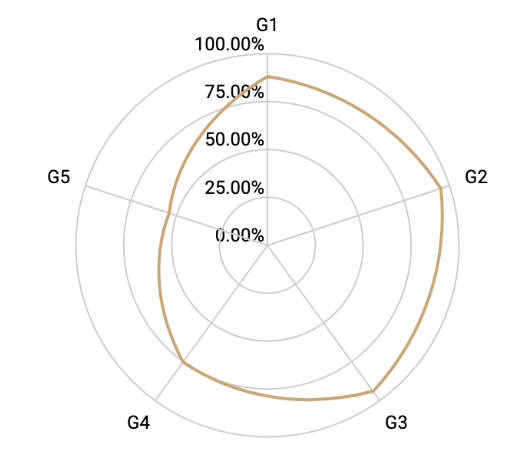
\includegraphics[width = 1 \columnwidth]{figures/guidelinereview.png}
    \caption{Web Graph of Heuristic Review on Guidelines}
    \label{fig:guidelinereview}
\end{figure}

\begin{figure*}[h]
    \centering
    \includegraphics[width = 2 \columnwidth]{figures/"IT1 codeblocks results".png}
    \caption{Differences in Codeblock outputs between novice and experienced programmers while doing the same machine learning task}
    \label{fig:codeblockdifference}
\end{figure*}


\subsection{Prototype Features Discovered}

During each iteration, specific limitations and problems were discovered while the user was testing the system. The first limitation that was discovered was during the first iteration testing using the iteration of design made using Gravit. Some users mentioned that there were blocks missing that was needed in order to create a proper linear regression system. The blocks that were mainly recommended was the train and test split block as well as proper testing blocks needed to determine the accuracy and behavior of the regression system created. These blocks were later added in the second iteration of the system. The train and test split block was responsible for splitting the current dataset into X and Y train and test sets respectively. Respective output blocks were also added to check the coefficients, mean squared error, and R squared score. The tool uses the Scikit-learn Metrics library to compute for these output values.

The second iteration brought about the first iteration with a functional prototype that was used during the iteration testing. However, there were several limitation using the Blockly environment. The limitations were the lack of regression visualization and error handling during this iteration as well as missing codeblocks needed to create or customize the system with each being addressed in the next iteration. The regression visualization was added as part of the three (3) main sections of the dashboard of the tool. Extensive error handling was also implemented to catch errors using the Python engine as well as custom errors that can be triggered through misuse of code blocks in the Blockly environment. The users also recommended codeblocks such as the import libraries block that was responsible for importing all necessary libraries needed to run the system as well as implementing a print block that could display certain values while testing. 

\subsection{Success and Completion Rates}

\begin{figure}[t]
    \centering
    \includegraphics[width = 1 \columnwidth]{figures/"IT2 success rate".png}
    \caption{Success rate for Iteration 2 Tasks.}
    \label{fig:it2successrate}
\end{figure}

For iteration 2, only two (2) tasks that creates Linear Regression models were given. One which involved coding or sorting code cells in a Google Colaboratory Notebook, and the other using the iML tool. Each of these tasks were counter balanced. As seen in figure \ref{fig:it2successrate}, for the notebook task all participants were able to complete it as the coding environment was something familiar for the participants to use. 

On the other hand, when using the iML tool 30\% of the participants failed the task, as indicated by the red portion of figure \ref{fig:it2successrate} since some were unfamiliar with using code blocks and the overall environment was a new approach for them to create Linear Regression models. The participants that failed the iML tool task were mostly those that received the tool as their first task.

\begin{figure}[t]
    \centering
    \includegraphics[width = 1 \columnwidth]{figures/"IT3 success rate".png}
    \caption{Setup for Usability Testing}
    \label{fig:it3successrate}
\end{figure}

Iteration 3 had varied tasks that involved improving the accuracy of a the Linear Regression model using two (2) different datasets for scenario 1 and 4, and tasks that would align the visualization of the tool around the zero-point for scenario 2 and 3. 

Overall most participants were able to complete all tasks, as seen in figure \ref{fig:it3successrate} with scenario 4 receiving a 100\% completion rate. Since all these tasks were counterbalanced, by the time scenario 4 was accomplished, the participants had sufficiently explored the iML tool to be able to complete each task. Scenario 2 and 3 have partial passes, as indicated by the yellow portions of figure \ref{fig:it3successrate}, this means that the participants were able to partially complete building their Linear Regression model but decided to skip the task since they could not identify what set of blocks to use next. 

\section{Discussion}

Figure \ref{fig:guidelinereview}, shows the guidelines review that was done after iteration 3. The closer the web is towards the outer circle, the more the guideline is adhered to. Thus, the current iML tool created mostly adhered to guidelines 1-4 related to system interaction and visualization. 

Guideline 5 had mixed results from the iteration 3 participants as some participants are still looking for more descriptive errors. 

User activity flow patterns were observed in iteration 2 since the focus of the tests were on the discoverability of the iML tool's features. For the novice users, the common user activity flow pattern observed was Explore-Edit-Guess as these users took the time to explore the sandbox iML environment before forming the Linear Regression model. Experienced users were observed to follow Edit-Explore-Guess as they are familiar with the ML terminologies they would assemble the model and edit it as they explore the tool. The patterns were decided by observing screen recordings of iteration 2 and deciding the order of activity done. An interrater reliability score was used to determine the patterns, 60\% was the acceptable agreement level. The agreement of Explore is 63.33\%, Edit is 56.67\% and Guess is 73.33\%.

We were able to design guidelines that affected the interface of our interactive prototype. These are discussed in the next section. 

\section{Design Guidelines Implications}

\subsection{Initial System Design}
We began with an initial idea of the prototype which was used in the first round of usability tests. The focus was on designing a prototype that will allow a typical user to interact with codeblocks as opposed to writing text-based programs. It should be noted that the first iteration was not intended to be a functional tool. The objectives of the prototype can be separated into three (3) distinct categories, namely: Interaction Focus, Intended Product, and Concept Flexibility. The first category focused the interaction of the system with the user and the code blocks. The next category covered the intended product itself and the features it can offer to the user. The last category focused on the flexibility of the codeblocks and how the user will interact with these blocks. Each category corresponds to a design factor according to the research conducted by \citeA{amershi2011designing}.
\begin{figure}[t]
    \centering
    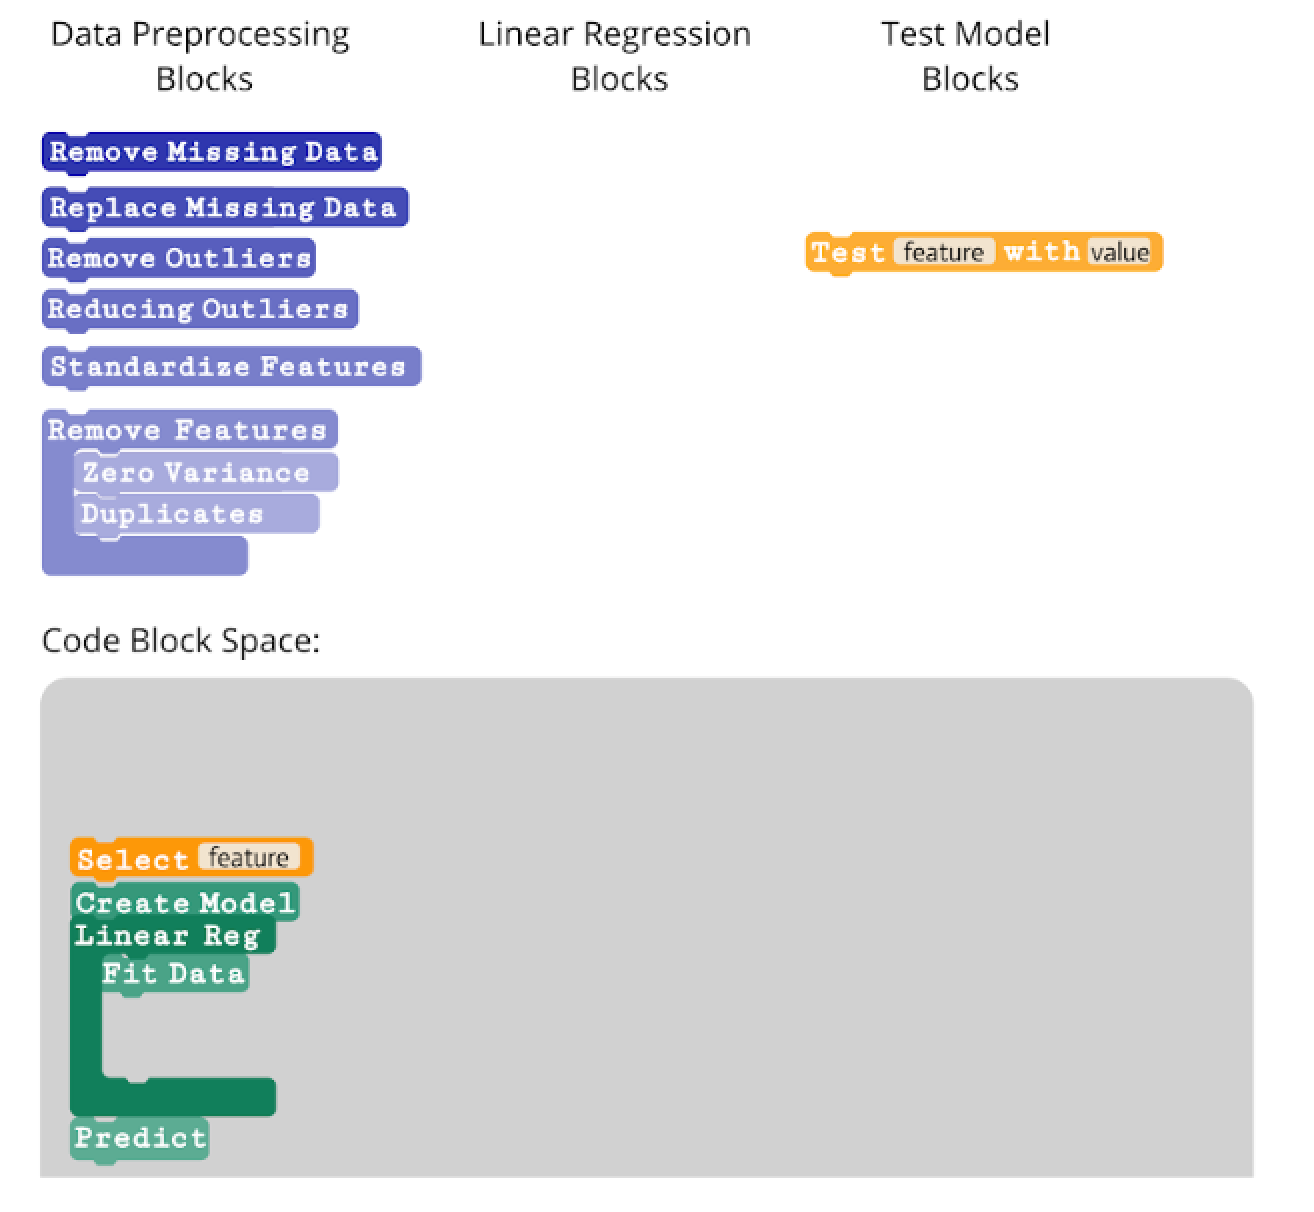
\includegraphics[width = 1 \columnwidth]{figures/IT1_full}
    \caption{Preview of the Codeblock Design in the Initial Version (Iteration 1) of the Prototype. The blocks are sorted and grouped depending on their use. These are also color-coded per category. }
    \label{fig:it1}
\end{figure}
This said prototype was drafted using Gravit, an online multi-platform design application which allows the user to drag, drop, and clip vectors together, simulating the experience of using code blocks as seen on figure \ref{fig:it1}. The initial set of code blocks are separated into three (3) categories, namely: the Data Preprocessing blocks, the Linear Regression blocks, and the Testing blocks, each representing the color purple, green, and orange respectively as seen in figure \ref{fig:it1}. Each category represents a phase in the machine learning pipeline with intended to provide the user with the basic set of functions needed to create and test a simple linear regression system as well as incorporating commonly used data preprocessing features.

\subsection{Improved System Features}
Following the multiple iterations of usability tests, we managed to extract insights and behaviours that allowed us design a functional prototype that understood novice programmers. 
We now introduced significant changes as we improved the prototype thru each iteration. The prototype was designed to be a web application built using Google's Blockly library. Blockly creates an environment that allows code snippets from common programming languages to be represented as code blocks which allows developers to create custom code blocks with their respective code generators for each of the supported programming languages. However, Blocky does not run the code generated by the code blocks, but is able to output the code generated in a formatted string. With this limitation in mind, we integrated Django to compile and run the generated code. The output of the Python program is then passed through a JSON object and then displayed in the output text box. This allows a transition between assembling the code blocks and having a code output that the novice programmer can use as basis for their work. 

\begin{figure*}[t]
    \centering
    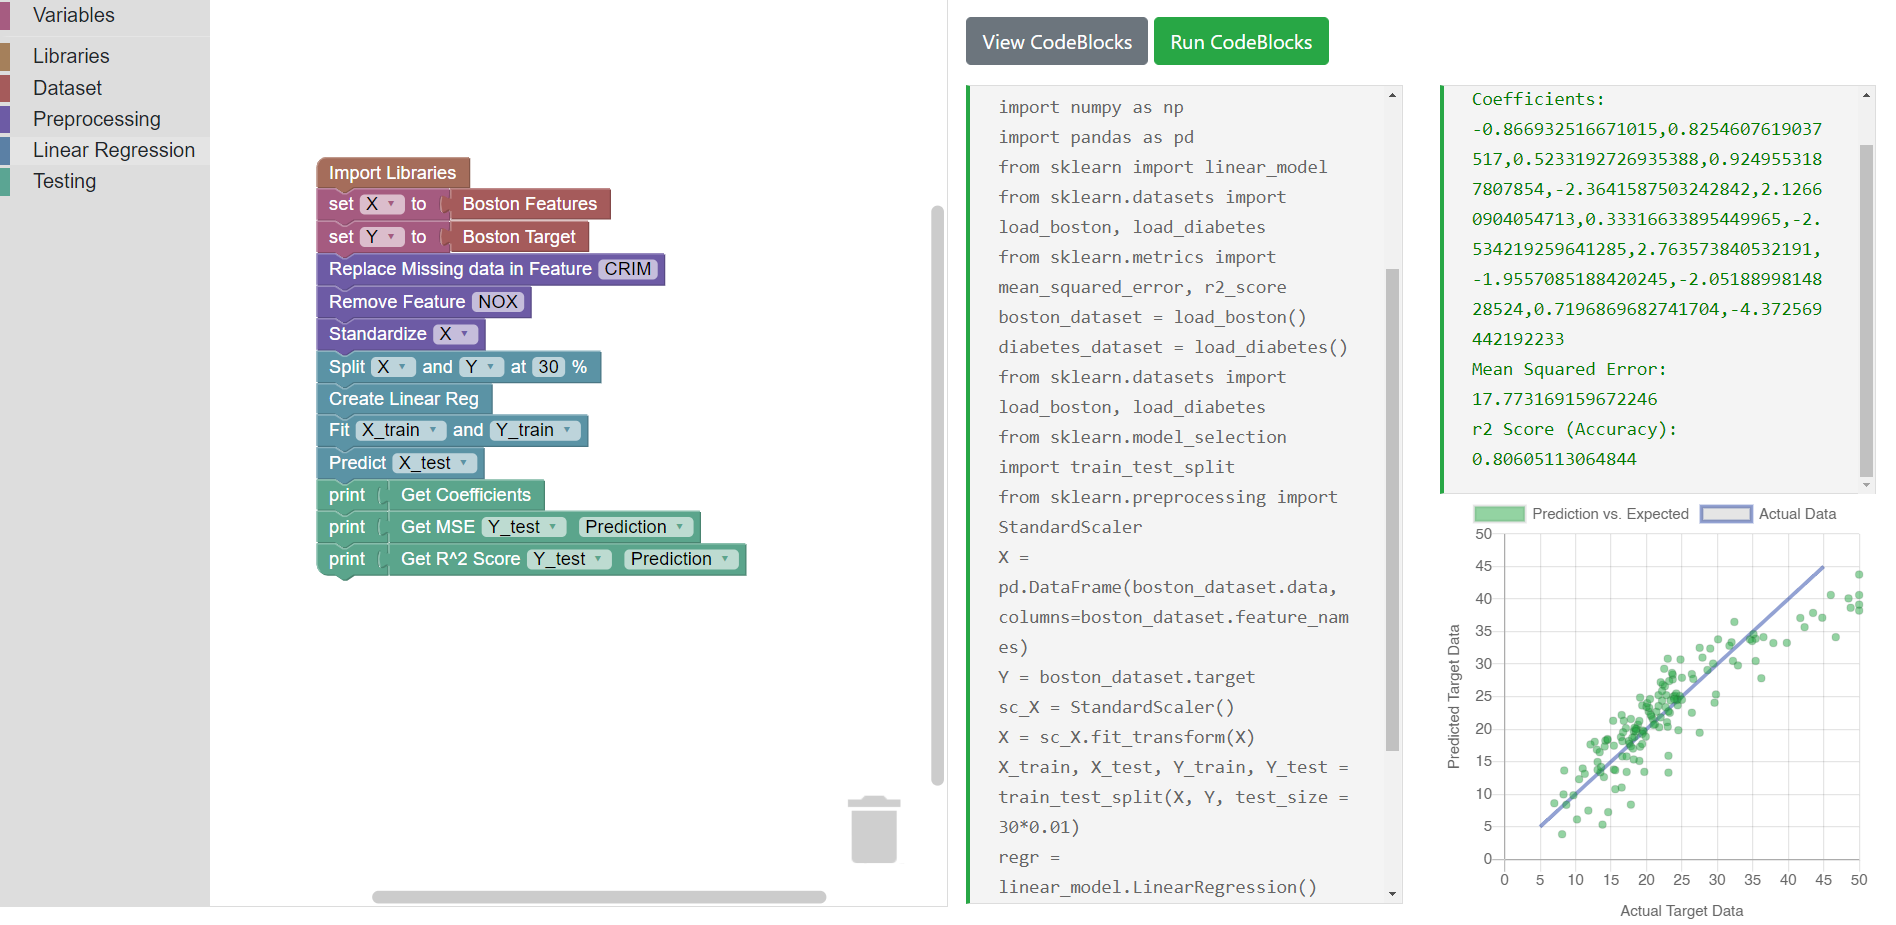
\includegraphics[width = 2 \columnwidth]{figures/Gen_Interface}
    \caption{General Interface and Environment of the Sandbox Workspace Prototype}
    \label{fig:gen_interface}
\end{figure*}

TREX is the result of the final iteration testing and was designed to be a web-based interactive tool that aims to provide the user with a sandbox environment for testing and creating Linear Regression Machine Learning Systems that can be used on various datasets. All functions of the tool can be accessed in the main dashboard that is separated into three main sections, each with a specific goal in mind as seen on figure \ref{fig:gen_interface}. The three main sections are the Sandbox Environment section, Code Translation and Output section, and the Regression Visualization section.
\begin{comment}
\begin{figure}[t]
    \centering
    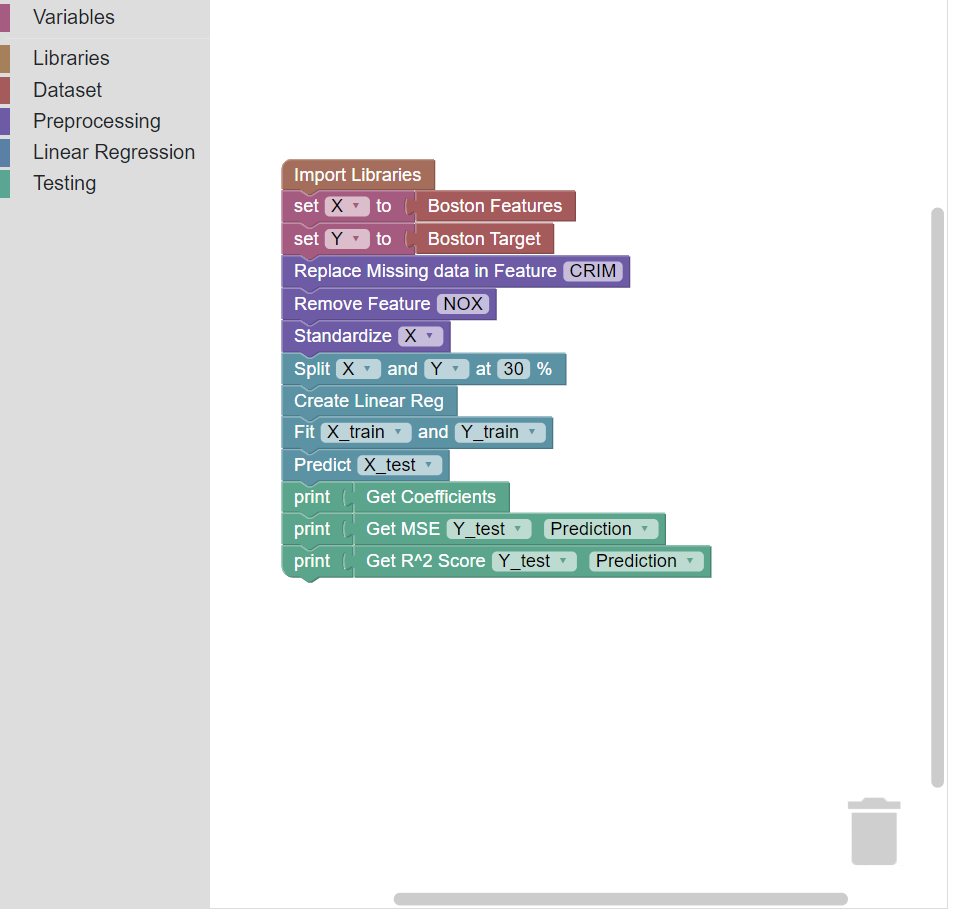
\includegraphics[width = 1 \columnwidth]{figures/Sandbox}
    \caption{TREX Sandbox Environment toolbox and workspace}
    \label{fig:sandboxenv}
\end{figure}
\end{comment}
The sandbox section includes the environment where the user can create their own linear regression system using the various code blocks provided by the tool. The environment consists of two major components the toolbox and the workspace. The toolbox holds and stores all code blocks needed to create your own linear regression system while the workspace is used for arranging the blocks that represents the code for the system. The user will be able to drag and drop code blocks from the toolbox onto the workspace which can then be clipped or snapped to other code blocks, as well as edit the various parameters found on the code blocks themselves as seen in figure \ref{fig:sandboxenv}. The user may be able to delete code blocks by dragging them into the bin icon on the lower-left side of the workspace which can also view previously deleted code blocks when left-clicked.

\begin{figure}[]
    \centering
    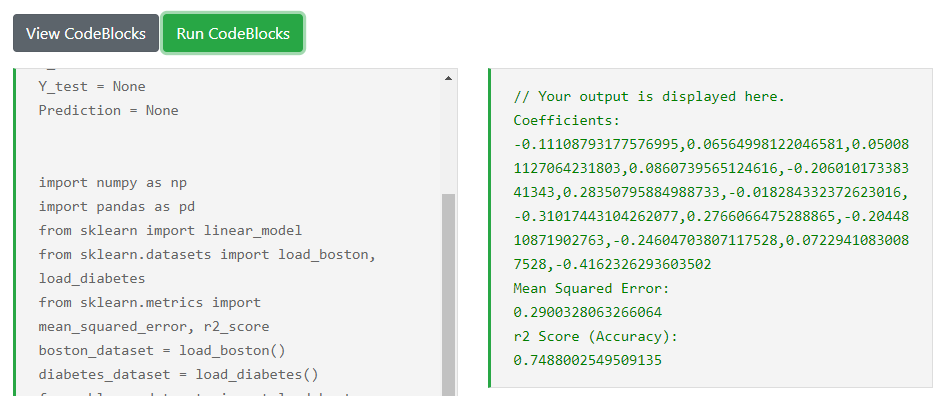
\includegraphics[width = 1 \columnwidth]{figures/Code_Output}
    \caption{Snippet of the Code Translation and Output Section}
    \label{fig:codeout}
\end{figure}

The code translation and output section is responsible for displaying the translated code from the code blocks arranged in the workspace and the respective outputs when run as seen in figure \ref{fig:codeout}. The View CodeBlocks button will parse each code block in the workspace from top to bottom in a linear fashion and displayed in the code display on the left side of the section. The Run CodeBlocks button will then run the parsed Code Blocks using a Python compiler with each output display on the output display on the right side of the section. To parse the code blocks, the tool converts the visual code blocks into actual code snippets which are then arranged based on the order of the blocks. Because of this, all variables are first initialized to a default value to make sure that there will be no null values. The code snippets will then be concatenated into a formatted string which is then displayed on the output display section.

\begin{figure}[t]
    \centering
    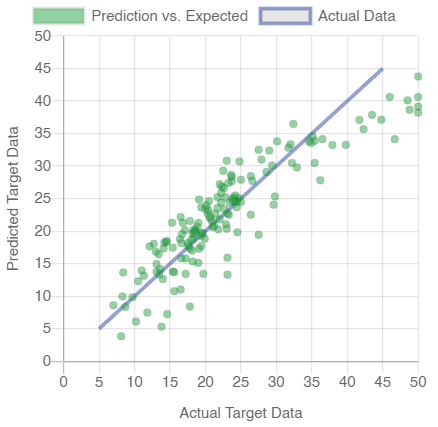
\includegraphics[width = 1 \columnwidth]{figures/Reg_Vis}
    \caption{Regression Visualization Section in the Sandbox Prototype}
    \label{fig:regvis}
\end{figure}

The regression visualization section is responsible for displaying the predicted target data in comparison with the actual target data as well as the diagonal line descriptor of the system created as seen in figure \ref{fig:regvis}. The tool first selects the two data arrays it will be using which is a combination of either the train or test set of Y and the Prediction based on the shape the prediction and the train or test set(if they match). It then plots a line based on the regression equation of the given target feature. The tool uses the Chart.js library to create a mixed linear and scatter graph to show the data as well as the plotted line.

\section{Limitation and Future Work}

One of the areas that can be explored in the future is the potential use of more complex machine learning algorithms with visual programming or the concept of a sandbox environment. With the amount of machine learning libraries found that is being supported on Python, each function can be translated into specific code blocks. However, there are limitations with the current iteration of the tool. One of these limitation has to do with the the current implementation of the datasets being used with the tool. The current iteration uses premade datasets retrieved from the Scikit-learn sample datasets library due to how they are structured and the overall cleanliness of the dataset. Some codeblocks assume that the dataset being used on the system are structured in a specific way before they are processed and fitted onto the machine learning algorithm. If the dataset does not follow this specific structure, it is possible that the tool may wrongly interpret the data being given to it. This may result in an unstable system or falsely interpreted data results. 

In addition, better ways of gaining user activity flow can be explored in the future by using system logs for more accurate tracking of user activity flows. It may make patterns more evident compared to annotation and observation alone. For the guidelines, future work could include exploring if the design guidelines discovered from our prototype can be applied to other machine learning algorithms especially how they may change depending on the objective and use of the algorithm. 

\section{Conclusion}
As interactive machine learning platforms are becoming more in demand, it is important to understand the human factors that influence the design of these systems. We echo the findings of \cite{sarkar2015interactive} and confirm the guidelines we derived following the methodologies of \cite{amershi2011designing} that novice programmers are less more confident that their experienced counterparts. We found that they tend to explore first their environment before diving into building their solution as seen from our regression experiments. From these observations, we validated our guidelines through a heuristic review and software usability scores. These findings and implications emphasize the dynamic and growing demand for better design in interactive machine learning systems. With further research, we can still investigate and validate whether these behaviours are observable as well in other machine learning activities beyond regression experiments. 


% \begin{table}
%   \centering
%   \begin{tabular}{l r r r}
%     % \toprule
%     & & \multicolumn{2}{c}{\small{\textbf{Test Conditions}}} \\
%     \cmidrule(r){3-4}
%     {\small\textit{Name}}
%     & {\small \textit{First}}
%       & {\small \textit{Second}}
%     & {\small \textit{Final}} \\
%     \midrule
%     Marsden & 223.0 & 44 & 432,321 \\
%     Nass & 22.2 & 16 & 234,333 \\
%     Borriello & 22.9 & 11 & 93,123 \\
%     Karat & 34.9 & 2200 & 103,322 \\
%     % \bottomrule
%   \end{tabular}
%   \caption{Table captions should be placed below the table. We
%     recommend table lines be 1 point, 25\% black. Minimize use of
%     table grid lines.}~\label{tab:table1}
% \end{table}



%
\balance{}


% BALANCE COLUMNS
\balance{}

% REFERENCES FORMAT
% References must be the same font size as other body text.
\bibliographystyle{SIGCHI-Reference-Format}
\bibliography{myreferences}

\end{document}

%%% Local Variables:
%%% mode: latex
%%% TeX-master: t
%%% End:
